\setcounter{rownumber}{0}
\singlespacing
\chapter{Manuscript II: A coherently stimulated phonon spectrometer}
\label{chap:CABS}
\acresetall

%  Copy this file for each main chapter, make sure to add it to main.tex

% Example author list with footnote style affiliations
%
Joel N. Johnson\footnote{\label{CABS-NAU}
Department of Applied Physics and Materials Science, Northern Arizona University, Flagstaff, AZ 86011, USA
}$^,$\footnote{\label{CABS-MIRA}
Center for Materials Interfaces in Research and Applications, Flagstaff, AZ 86011, USA
},
Nils T. Otterstrom\footnote{\label{CABS-Sandia}
Sandia National Laboratory, 1515 Eubank Blvd SE, Albuquerque, NM 87123, USA
},
Peter T. Rakich\footnote{\label{CABS-Yale}
Department of Applied Physics, Yale University, New Haven, CT 06520, USA
},
Ryan O. Behunin$^\mathrm{\ref{CABS-NAU}}$$^,$$^\mathrm{\ref{CABS-MIRA}}$

\hfill

%  Extra copyright disclaimer to be safe
%
\textit{This is the Accepted Manuscript version of an article accepted for publication in Nature Photonics. Wiley Inc is not responsible for any errors or omissions in this version of the manuscript or any version derived from it. The Version of Record is available online at} \url{https://doi.org/}\textit{.}

\doublespacing

%%%%%%%%%%%%%%%%%%%%%%%%%%%Nature Photonics Format Requirements%%%%%%%%%%%%%%%%%%%%%%%%%%%%%%%%%%%
%Article
%An Article is a substantial novel research study, with a complex story often involving several techniques or approaches.

%Format

%Main text – up to 3,000 words, excluding abstract, Methods, references and figure legends.
%Abstract – up to 200 words, unreferenced.
%Display items – up to 6 items (figures and/or tables).
%Article should be divided as follows:
%Introduction (without heading)
%Results
%Discussion
%Online Methods. ​
%Results and Methods should be divided by topical subheadings; the Discussion does not contain subheadings.
%References – as a guideline, we typically recommend up to 50.
%Articles include received/accepted dates.
%Articles may be accompanied by supplementary information.
%Articles are peer reviewed.

%%%%%%%%%%%%%%%%%%%%%%%%%%%%%%%%%%%%%%%%%%%%%%%%%%%%%%%%%%%%%%%%%%%%%%%%%%%%%%%%%%%%%%%%%%%%%%%%%%
%  Chapter contents here

\section{Abstract}

\section{Introduction}
State of brillouin microscopy
Applications and usefulness
Challenges: selection of backscattered signal
  conflated with Stokes field
  phase-matching requires probe wavelength to be exactly that of Stokes
Wouldn't it be nice if we could break free of strict phase-matching requirements, therefore perfectly isolating the signal
In this work

  \subsection{Theory of CABS}
  description of physics with scattered power equation

  \subsection{Phase-matching at short lengths}
  phase-matching bandwidth description with equation

\section{Methods} % online-only for Nature Photonics

  \subsection{Theory of CABS}
  full CABS theory arriving at scattered power

  \subsection{Phase-matching bandwidth}
  phase-matching bandwidth theory

\section{Results}

  \subsection{Design of instrument}
  description of design
  figure: instrument
    apparatus design
    sensitivity measurements

  \subsection{From fiber-coupled to micrometer-scale free-space}
  figure: demonstration measurements
    1mm uhna3 fiber
    1mm CS2 bulk

    \begin{figure*}[t]
        \centering
        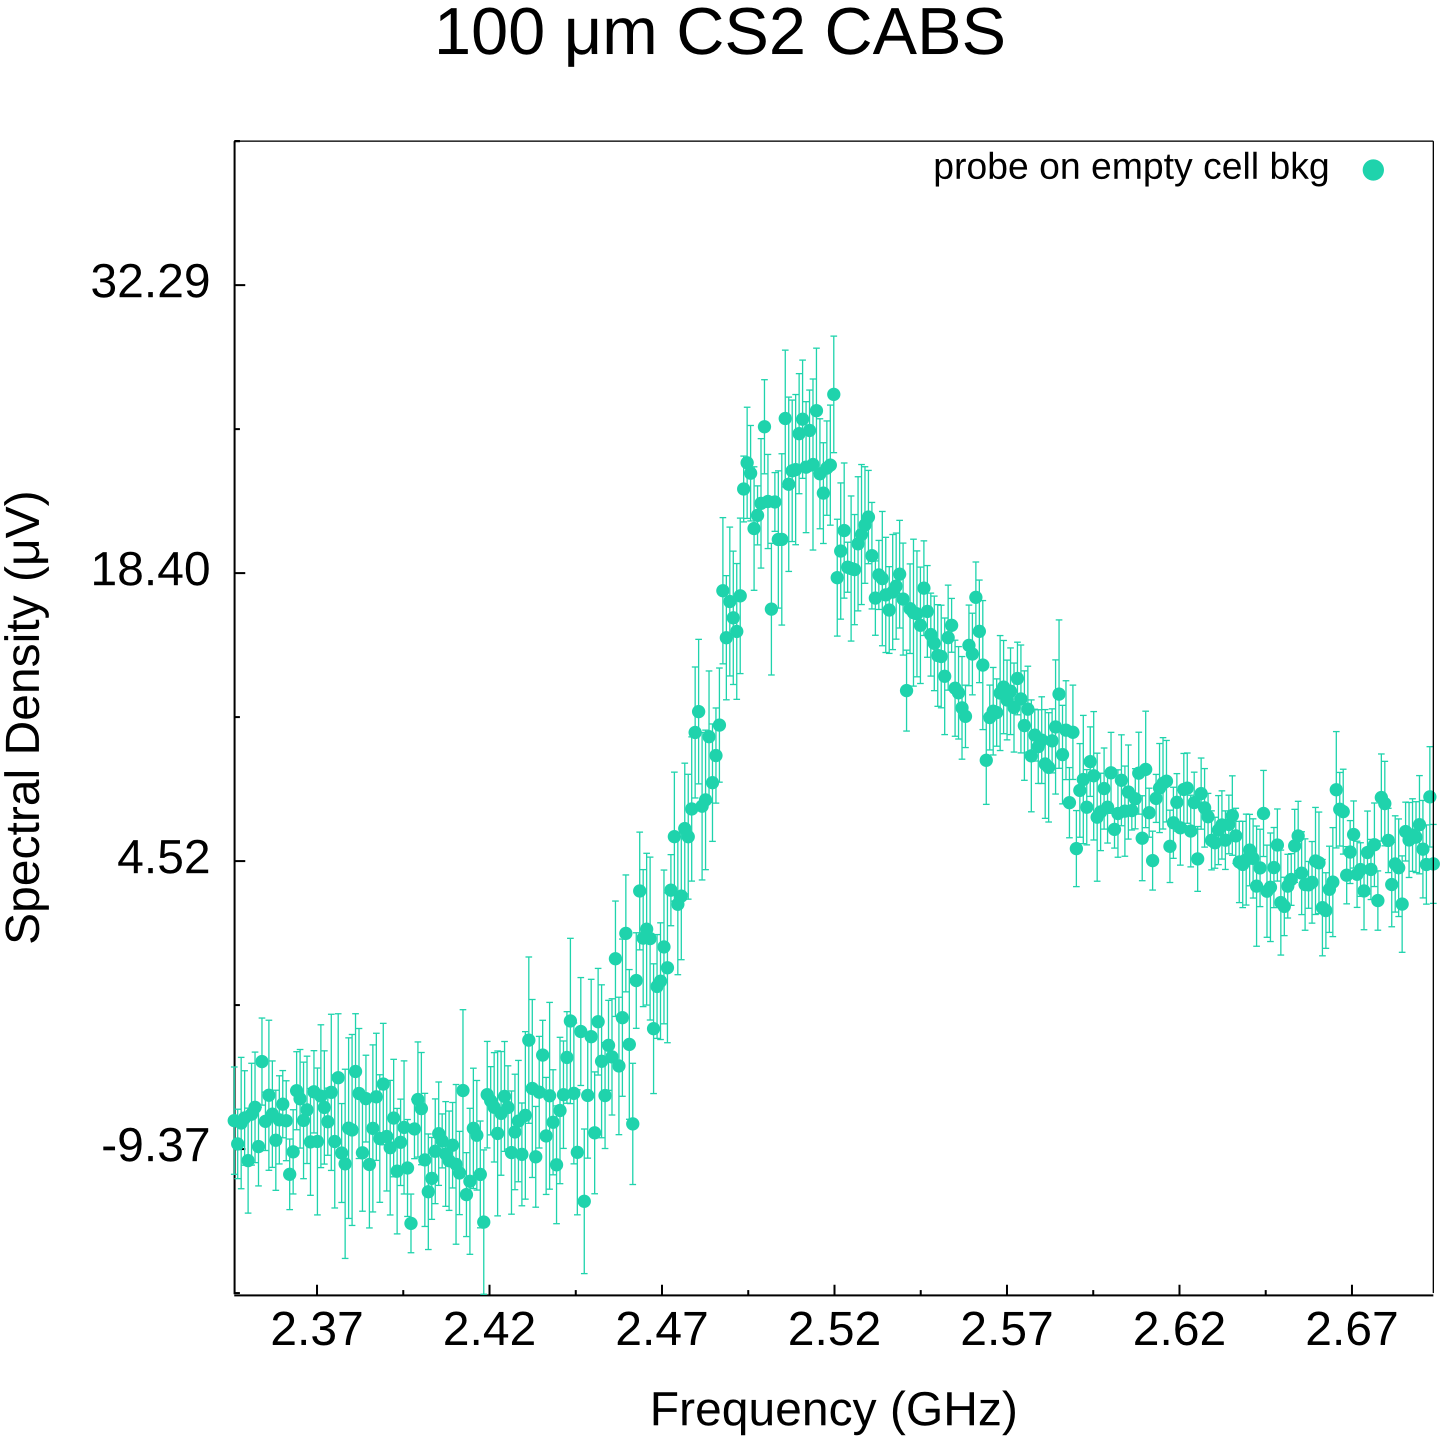
\includegraphics[width=\textwidth]{figs/4-CABS/CABS-100um CS2.png}
        \caption{CABS measurement of 100um of CS2.}
        \label{fig:CABS 100um CS2}
    \end{figure*}

    comparison to stimulated brillouin and spontaneous brillouin?

  \subsection{Relaxation of Phase-matching conditions}
  figure: phase-matching
    peak vs pump-probe separation 1cm uhna3, CS2
    peak vs pump-probe separation 1mm uhna3, CS2

\section{Discussion}

\section{Acknowledgements}

\section{Appendix}
  \subsection{Equal contribution of P, S, Pr}
  figure: P, S, Pr equal contributors
